\chapter{Media Item Deduplication}
\label{sec:media-item-deduplication}

% the code below specifies where the figures are stored
\ifpdf
    \graphicspath{{6_media_item_deduplication/figures/PNG/}{6_media_item_deduplication/figures/PDF/}{6_media_item_deduplication/figures/}}
\else
    \graphicspath{{6_media_item_deduplication/figures/EPS/}{6_media_item_deduplication/figures/}}
\fi

\section{Introduction}

In the previous \autoref{cha:media-item-extraction}
in \autoref{sec:the-need-for-media-item-deduplication},
we have motivated the need for media item deduplication.
By clustering media items, we get a~higher level view on
a~media item cluster's overall performance on different networks.
As detailed in \autoref{sec:definition}, media items can be
photos or videos.
WordNet~\cite{fellbaum1998wordnet,miller1995wordnet} defines
the term \emph{duplicate} as
\textit{``a copy that corresponds to an original exactly''}.
the corresponding verb \emph{to duplicate} is defined as to
\textit{``make a duplicate or duplicates of''}.
The derived term \emph{deduplication} in consequence refers to
the act of eliminating duplicate or redundant information.

\subsection{Definition of Exact Duplicate for Photos}

We define two media items of type photo as \emph{exact duplicate},
if their pixel contents are exactly the same.
This implies that by our definition, a scaled version
of the same photo is \emph{not} an exact duplicate. 
Similarly, a rotated version of a photo is also \emph{not}
an exact duplicate. 
In contrast, two photo files with different file names,
or different Exchangeable image file
format\footnote{\url{http://www.cipa.jp/english/hyoujunka/kikaku/pdf/DC-008-2010_E.pdf},
accessed November 22, 2012}
(Exif) data, are considered exact duplicate,
if their pixel contents are exactly the same.
Exact duplicate photos typically occur if users share content 
from one social network on another, for example,
if one user posts a photo on Instagram that then someone else
(or even the same user) posts on Facebook.

\subsection{Definition of Near-Duplicate for Photos}

We define two media items of type photo as \emph{near-duplicate},
if their pixel contents differ no more than a given threshold.
Examples of near-duplicate photos are scaled versions
of the same photo, photos shot from a slightly different angle,
rotated photos up to a certain degree, \emph{etc.}
Near-duplicate photos typically occur if event attendants
stand close to each other and thus take photos
from a similar standpoint.
Another scenario is a user applying a photo effect to a photo
(like an Instagram filter) and then sharing both, the modified,
and the unmodified version.

\subsection{Definition of Exact Duplicate for Videos}

We define two media items of type video as \emph{exact duplicate},
if their pixel contents are frame by frame exactly the same.
In practice, we lower this condition and instead of every frame
only consider frames at shot boundaries.
We make \emph{no} requirements on the audio, \emph{i.e.},
a video in two different languages, however, that fulfills the 
pixel contents equality condition, is considered exact duplicate.
Typical scenarios where exact duplicate videos can occur is,
for example, two users sharing the same YouTube video
independently from each other.

\subsection{Definition of Near-Duplicate for Videos}

We define two media items of type video as \emph{near-duplicate},
if their pixel contents per frame differ no more
than a given threshold.
In practice, we lower this condition and instead of every frame
only consider frames at shot boundaries.
Typical scenarios where near-duplicate videos can occur is through
logo or subtitle insertion, resizing, re-encoding,
or aspect-ration changes.
Note, we do not consider video subsegments near-duplicates.

\subsection{Special Case of Photo Contained in a Video}

We define the special case of
\emph{a photo being contained in a video} if the pixel contents
of a photo media item differ no more than a given threshold from
the pixel contents of any of the frames of a video media item.
In practice, we lower this condition and instead of every frame
only consider frames at shot boundaries.
Typically, this phenomenon occurs if two event attendants
of the same event both cover the event from almost the same
standpoint, however, if the one attendant takes a video,
while the other attendant takes a photo.

\section{Related Work}
\label{sec:related-work}

Another relevant work area is duplicate and near-duplicate media detection. Work on ordinal measures for image correspondence started in the last decade of the 20\superscript{th}~century~\cite{Bhat}. Recently, Chum \emph{et al.} have proposed a near-duplicate image detection method using MinHash and tf--idf weighting~\cite{Chum}. A~method for both photos and video has been proposed by Yang \emph{et al.}~\cite{Yang}. Specialized methods for video exist as well~\cite{Min, Wu}, an excellent survey of which has been conducted by Lian \emph{et al.}~\cite{Lian}.



\section{Photo Deduplication}
\subsubsection{Media Item Deduplication}
We try to evaluate the popularity of the media items shared across social networks. This task involves the deduplication of extracted media items.
For photos, we use PhotoSweeper\footnote{\url{http://itunes.apple.com/us/app/photosweeper/id463362050?mt=12}}, a commercial photo deduplication software and we have manually deduplicated videos. In the future, we aim to perform this task fully automatically but with this work, we have already created a baseline for specific future algorithms tailored to media item deduplication on social networks.

\paragraph{Photo Deduplication}
The photo duplication software we employed allows for different algorithms to be used. We have applied strict pixel-per-pixel comparison for the detection of \emph{exact} duplicates, i.e. we do \emph{not} count a resized version of a photo as exact duplicate. Based on bitmap- or histogram-based similarity comparison methods, we introduce the relatively wide term of \emph{loose} duplicate. Bitmap similarity is based on comparing pixels of size-reduced bitmaps.
For our comparison, we used bitmaps of the size $128 \times 128$ pixels without smoothed edges, which corresponds to the best quality settings in the software.
Histogram similarity is based on comparing histograms of size-reduced bitmaps. This method helps finding similar photos despite differences in color saturation and lighting. For both similarity comparison methods, a varying threshold was used. In our experiments, we could not make out a clear winning setting for all events. Rather, even for the same event, only a combination of both similarity comparison methods led to satisfactory results, i.e. to a set of loosely duplicate photos that also a human being would have chosen. We would like to highlight, however, that all detected loosely duplicate photos were detected algorithmically, which is an important fact for the objective of fully automating the deduplication process.

\paragraph{Video Deduplication}
We have deduplicated the videos in the dataset by first automatically splitting them in shots~\cite{CrowdsourcingEvent}, and then manually comparing the videos shot-wise. We considered \emph{exact} duplicates the videos that shared the same shots and same length. For \emph{loose} duplicates, we manually decided whether the videos showed loosely the same based on human judgment. We do not claim that our results are algorithmically reproducible for loosely similar video detection.

\section{Video Shot Detection}
Video shot detection is the processor-intensive task of splitting a~video into continuous shots, with hard or soft cuts as the boundaries. In this paper, we present a~client-side on-the-fly approach to this challenge based on modern HTML5-enabled Web APIs. We show how video shot detection can be seamlessly embedded into video platforms like YouTube using browser extensions. Once a~video has been split into shots, shot-based video navigation gets enabled and more fine-grained playing statistics can be created.

\subsection{Introduction}
Official press statistics~\cite{youtube:stats} from YouTube, one of the biggest online video platforms, state that more than 13 million hours of video were uploaded during 2010, and that 48 hours of video are uploaded every single minute. Given this huge amount of video content, it becomes evident that advanced search techniques are necessary in order to retrieve the few needles from the giant haystack. Closed captions allow for keyword-based in-video search, a~feature announced in 2008~\cite{googlevideo}. Searching YouTube for a~phrase like ``that's a~tremendous gift'', a~caption from Randy Pausch's famous last lecture \emph{Achieving Your Childhood Dreams}\footnote{Last Lecture: \url{http://bit.ly/pausch-last-lecture}}, reveals the video of his lecture. If no closed captions are available, nor can be automatically generated, keyword-based search is still available over tags, video descriptions, and titles. Presented with a~potentially long list of results, preview thumbnails based on video still frames help users decide on the most promising result. YouTube uses an unpublished computer vision-based algorithm for the generation of smart thumbnails on YouTube and lets video owners choose one out of three automatically suggested thumbnails.

In this part of the thesis, we introduce on-the-fly shot detection for YouTube videos as a~third means besides keyword-based search and thumbnail preview for deciding on a~video from the haystack. As a~user starts watching a~video, we detect shots in the video by visually analyzing its content. We do this with the help of a~browser extension, i.e., the whole process runs dynamically on the client-side, using modern HTML5 JavaScript APIs of the \texttt{<video>} and \texttt{<canvas>} elements~\cite{Hickson2011}. As soon as the shots have been detected, we offer the user the choice to quickly jump into a~specific shot by clicking on a~representative still frame. \autoref{fig:screenshot} shows the seamless integration of the detected shots into the YouTube website enabled by the browser extension. The main contributions of this paper are the browser extension itself and improved video navigability by shot navigation. A~screencast\footnote{Screencast: \url{http://bit.ly/filmstrip}} and demo\footnote{Demo: \url{http://bit.ly/filmstrip-debug}} of our approach are available.

\begin{figure}
\begin{center}
   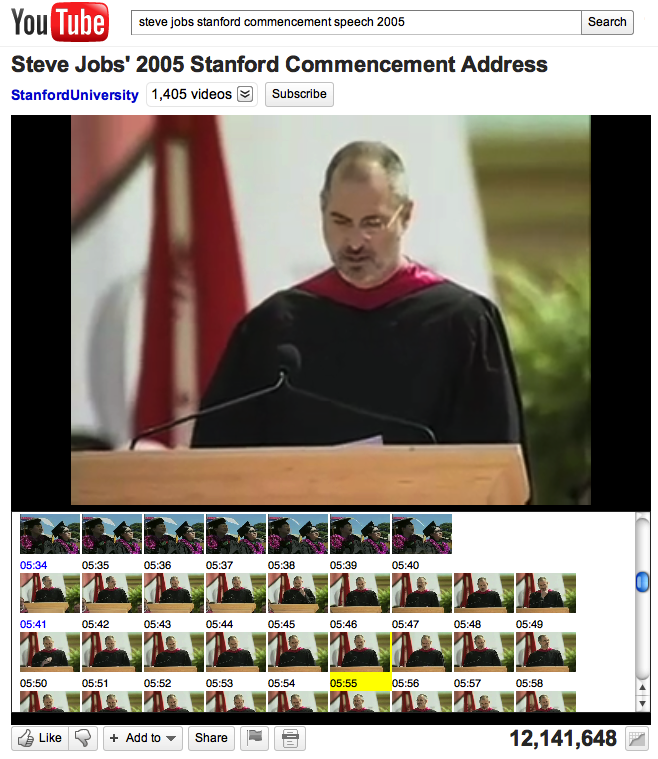
\includegraphics[width=0.8\linewidth]{./stevejobs.png}
\end{center}
   \caption{Screenshot of the browser extension running on YouTube, showing different detected shots.}
\label{fig:screenshot}
\end{figure}

\subsection{Related Work} \label{sec:related-work}
Video fragments consist of shots, which are sequences of consecutive frames from a~single viewpoint, representing a~continuous action in time and space. The topic of shot boundary detection has already been described extensively in literature. While some specific issues still remain (notably gradual transitions and false positives due to large movement or illumination changes), the problem is considered resolved for many cases~\cite{Hanjalic2002, Yuan2007}.
The contribution of our approach is that it is entirely Web-based and on-the-fly, which introduces interesting new challenges that traditional approaches do not have to cope with.
Highest shot detection accuracy can be reached with special command line tools, but therefore access to the hosting platform is needed, which in the general case is not given on the Web.
Our Web-based approach abstracts away most of the low-level details like the video codec, in favor for the high-level \texttt{<video>} API, however, this also comes at a~cost.
A~major issue is the uncertain streaming speed, where traditional approaches have immediate access to the video file on disk.
An additional challenge is the unknown key frame distribution of the target videos, which -- together with streaming speed issues -- makes exact frame-wise video navigation impossible.
Below, we present an overview of several well-known categories of shot detection techniques.

\emph{Pixel comparison methods}~\cite{Hampapur1994, Zhang1993} construct a~discontinuity metric based on differences in color or intensity values of corresponding pixels in successive frames. This dependency on spatial location makes this technique very sensitive to (even global) motion. Various improvements have been suggested, such as prefiltering frames~\cite{Zhang1995}, but pixel-by-pixel comparison methods proved inferior in the end and have steered research towards other directions.

A~related method is \emph{histogram analysis}~\cite{Smeaton1999}, where changes in frame histograms are used to justify shot boundaries. Their insensitivity to spatial information within a~frame makes histograms less prone to partial and global movements in a~shot. We argue as a~drawback that even visually very dissimilar frames can have similar overall histograms. For example, different shots in the same shot can be difficult to distinguish because of similar color information.

As a~compromise, a~third group of methods consists of a~\emph{trade-off between the above two techniques}~\cite{Ahmed1999}. Different histograms of several, non-overlapping blocks are calculated for each frame, thereby categorizing different regions of the photo with their own color-based, space-invariant fingerprint. The results are promising, while computational complexity is kept to a~minimum, which is why we have chosen a~variation on this approach in this paper.

Other approaches to shot boundary detection include the \emph{comparison of mean and standard deviations} of frame intensities~\cite{Lienhart1999}. Detection using other features such as edges~\cite{Zabih1995} and motion~\cite{Bouthemy1997} have also been proposed. However, Gargi \emph{et~al.}\ have shown that these more complex methods do not necessarily outperform histogram-based approaches~\cite{Gargi2000}. A~detailed comparison can be found in Yuan~\emph{et~al.}~\cite{Yuan2007}.
At time of writing, YouTube is about to roll out
a~similar native feature, however, frame-based and not shot-based as our approach\footnote{\url{http://youtube-global.blogspot.com.au/2012/03/looking-ahead-in-youtube-player.html}}.

\subsection{Shot Detection Algorithm} \label{sec:details-of-algo}
In this Section, we discuss our shot detection algorithm, which falls in the category of histogram-based algorithms.  Since visually dissimilar video frames can have similar overall histograms, we also take local histograms into account. 
We therefore split video frames in freely configurable rows and columns, i.e., lay a~grid of tiles over the frames. The user interface (\autoref{fig:algorithm}) currently allows for anything from a~$\mathit{1} \times \mathit{1}$ grid to a~$\mathit{20} \times \mathit{20}$ grid. For each step we examine a~frame $\mathit{f}$ and its direct predecessor frame $\mathit{f - 1}$.

Apart from the per-tile histogram average distance, the frame distance function further considers a~freely configurable number of \emph{most different} and \emph{most similar} tiles. This is driven by the observation that different parts of a~video have different intensities of color changes, dependent on the movements from frame to frame. The idea is thus to increase the influence of movements in the frame distance function, and to decrease the influence of permanence. In the debug view of our approach (\autoref{fig:algorithm}), blue boxes indicate movements, while red boxes indicate permanence. In the concrete example, Steve Jobs' head and shoulders move as he talks, which can be clearly seen by the blue boxes in the particular tiles. Additional movements come from a~swaying flag on the left, and a~plant on the right. In contrast, the speaker desk, the white background, and the upper part of his body remain static, resulting in red boxes. For this example, we use a~grid layout of $\mathit{20} \times \mathit{20}$ tiles ($\mathit{nTiles} = \mathit{400}$), and a~certain number $\mathit{tileLimit}$ of most different or similar tiles, i.e., we treat one third of all tiles as most different tiles, one third as normal tiles, and one third as most similar tiles, and apply boosting and limiting factors to the most different and most similar tiles respectively. This distribution was empirically determined to reveal best results. We work with also empirically determined values of~$\mathit{1.1}$ for the $\mathit{boostingFactor}$, which slightly increases the impact of the most different tiles, and $\mathit{0.9}$ for the $\mathit{limitingFactor}$, which slightly decreases the impact of the most similar tiles. The algorithm pseudo code can be seen in \autoref{code:algorithm}.

We define the average histogram distance between two frames $\mathit{f}$ and $\mathit{f - 1}$ as $\mathit{avgHisto}_{f}$. In a~first step, we have examined the histogram distance data statistically, and experimentally found out that while the overall average frame distance $\mathit{avgDist}_{f}$, defined as: $$\mathit{avgDist}_{f} = \frac{1}{\mathit{nTiles}}\sum_{t=1}^{\mathit{nTiles}}\mathit{avgHisto}_{f, t}$$ is very intuitive to human beings, far more value lies in the standard deviation $\mathit{stdDev}_{f}$, based on the definition of the overall average frame distance $\mathit{avgDist}_{f}$: $$\mathit{stdDev}_{f} = \sqrt{\frac{1}{\mathit{nTiles}}\sum_{t=1}^{\mathit{nTiles}}(\mathit{avgHisto}_{f, t} - \mathit{avgDist}_{f})^{2}}$$ We use the value of the standard deviation as a~value for the shot splitting threshold~\cite{Lienhart1999} to come to very accurate shot splitting results. We found the boosting and limiting factors to have overall a~positive quality impact on more lively videos, and a~negative quality impact on more monotone videos. Best results can be achieved if, after changing either the boosting or the limiting factors for the most similar or different tiles, the value of the shot splitting threshold is adapted to the new resulting standard deviation. The user interface optionally does this automatically.

\begin{figure}
\begin{center}
   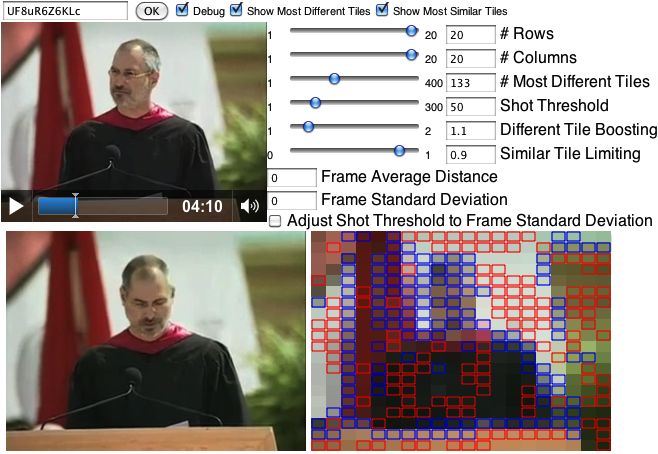
\includegraphics[width=1.0\linewidth]{./algorithm.png}
\end{center}
   \caption{Debug view of the shot detection process. Blue boxes highlight tiles with the most differences to the previous frame, red boxes those with most similarities.}
\label{fig:algorithm}
\end{figure}

\begin{lstlisting}[caption=Pseudocode of shot detection algorithm., label=code:algorithm, float]
for frame in frames
  f = frame.index  
  for tile in tiles of frame      
    avgHisto[f][tile] = getTilewiseDiff()
 
  mostDiffTiles = getMostDiffTiles(avgHisto[f])
  mostSimTiles = getMostSimTiles(avgHisto[f])
 
  for tile in tiles of frame    
    factor = 1  
    if tile in mostDiffTiles
      factor = boostingFactor
    else if tile in mostSimTiles
      factor = limitingFactor
    avgHisto[f][tile] = avgHisto[f][tile] * factor
  avgDist[f] = avg(avgHisto[f])
\end{lstlisting}

\subsection{Implementation Details} \label{sec:implementation}
Our shot detection algorithm is implemented in form of an extension for the Google Chrome browser. Chrome extensions are small software programs written in a~combination of HTML, JavaScript, and CSS, which users can install to enrich their browsing experience. For this paper we focus on extensions based on so-called content scripts. Content scripts are JavaScript programs that run in the context of Web pages via dynamic code injection. By using the standard Document Object Model (DOM), they can read or modify details of the Web pages a~user visits. The advantage of this browser extension approach is that it is very powerful and generalizable at the same time. Powerful in the sense that it allows for significantly changing ones user experience with a~platform like YouTube and simply add new features, and generalizable in the sense that in theory it would be possible to simply add video shot boundary detection to any HTML5-enabled video website.

The complete video analysis process happens fully on the client side. We use HTML5 JavaScript APIs of the \texttt{<video>} and \texttt{<canvas>} elements. The extension is activated as soon as the user enters a~YouTube video watch page. By default, YouTube uses Flash-encoded videos that are not programmatically accessible from a~JavaScript context, however, via an API used by the YouTube \texttt{<iframe>} embed code, we can replace the Flash version with the HTML5 version of a~video. In order to obtain a~video still frame from the \texttt{<video>} element at the current video position, we use the \texttt{drawImage()} function of the 2D context of the \texttt{<canvas>} element, which as its first parameter accepts a~\texttt{<video>} element. We then analyze the video frame's pixels tile-wise and calculate the histograms. In order to retrieve the tile-wise pixel data from the 2D context of the \texttt{<canvas>}, we use the \texttt{getImageData()} function. For processing speed reasons, we currently limit our approach to a~resolution of one second, i.e., for each analysis step seek the video in $\mathit{1s}$ steps. We then calculate the frame distances as outlined in \autoref{sec:details-of-algo}. For each frame, we generate an \texttt{<img>} element with a~base64-encoded data URI representation of the video frame's data that later gets injected into the DOM tree of YouTube, as can be seen in \autoref{fig:screenshot}. Each of the \texttt{<img>} elements has a~registered JavaScript event handler that upon click triggers two actions: first, the video seeks to the corresponding time, and second, the shot is tracked as a~hot spot in the video. Clicks on hot spots can be tracked using standard Web analytics services, which allows for the suggestion of more accurate entry points to videos in the longterm. 
In prior work~\cite{derive2011} we have shown how hot spots can be used to detect different kinds of events in videos.

\subsection{Evaluation} \label{sec:evaluation}
Detecting shots on-the-fly in streaming video comes with its very own challenges. First, it is a~question of streaming speed. We have to stream the same video twice in parallel: on the one hand the user-visible foreground video, and on the other hand the video used in the background for the analysis process. Especially with high-definition (HD) video this can be very demanding. We do not attach the background \texttt{<video>} element to the DOM tree to save some CPU cycles, however, the background video still needs to be seeked to each frame in second-steps and be processed, while the foreground video is playing normally. Even on a~higher-end computer (our experiments ran on a~MacBook Pro, Intel Core 2 Duo 2,66 GHz, 8 GB RAM), the process of analyzing and displaying in parallel a~$\mathit{1280} \times \mathit{720}$ HD video of media type \emph{video/mp4; codecs="avc1.64001F, mp4a.40.2"} causes an average CPU load of about 70\%. The HTML5 specification states that \textit{``[\ldots] when the playback rate is not exactly 1.0, hardware, software, or format limitations can cause video frames to be dropped [\ldots]''}~\cite{whatwgvideo}. In practice, this causes the analysis environment to be far from optimal. In our experiments we differentiated between false positives, i.e., shot changes that were detected, but not existent, and misses, i.e., shot changes that were existent, but not detected. Compared to a~set of videos with manually annotated shot changes, our algorithm detected fewer false positives than misses. The reasons were gradual transitions and shots shorter than one second (below our detection resolution) for misses, and large movements in several tiles for false positives. Overall, we reached an accuracy of about 86\%, which is not optimal, but given the challenges sufficient for our use case of facilitating in-video navigation. 
Performance potential resides in the usage of Web Workers,
JavaScript programs that run in the background, independently of other user interface scripts.

\subsection{Future Work and Conclusion} \label{sec:future-work-conclusion}

In a~first step, future work will consist in improving the analysis speed by dynamically selecting lower quality analysis video files, given that videos are available in several resolutions (both LD and HD). We will check in how far analysis results differ for the various qualities. In a~second step, we will work on more advanced heuristics for the various user-definable options in the analysis process (\autoref{fig:algorithm}). While there is no optimal configuration for all types of videos, there are some key indicators that can help categorize videos into classes and propose predefined known working settings based on the standard deviation $\mathit{stdDev_{f}}$ and the overall average frame distance $\mathit{avgDist_{f}}$. Both are dependent on the values of $\mathit{boostingFactor}$, $\mathit{limitingFactor}$, $\mathit{rows}$, and $\mathit{columns}$. Interpreting our results so far, there is evidence that low complexity settings are sufficient in most cases, i.e., a~number of $\mathit{rows}$ and $\mathit{columns}$ higher than~$\mathit{2}$ does not necessarily lead to more accurate shot detection results. The same applies to the number of to-be-considered most different or similar tiles $\mathit{tileLimit}$. We even had cases where not treating those tiles differently at all, i.e., setting $\mathit{boostingFactor} = \mathit{limitingFactor} = \mathit{1}$, led to better results. We plan to use an adapted version of the algorithm for event summarization based on user-generated video content.

Concluding, we have promising results, especially in combination with hot spot identification from prior work~\cite{derive2011}, which in future can provide for more accurate entry point suggestions in long videos, or enable skip marks in videos with intros.
For video shot detection, some challenges remain, especially with the observed streaming speed-related issues and predefined parameter settings to improve accuracy. None\-theless, when searching for a~certain point in a~video, the obtained results already allow for focused in-video navigation and also facilitate exploratory shot-wise video consumption.

\section{Video Deduplication}

\section{Evaluation}

\section{Conclusion}

\section*{Chapter Notes}
This chapter is partly based on the following publications:
\todo{Add publications}